This section discusses the implementation of the algorithm, the problems encountered and a comparison with the latest Cuckoo version.

\subsection{Implementing the algorithm}

What follows is a short overview of how the algorithm was implemented, the actual code can be found on GitHub\footnote{\url{https://github.com/MartijnB/cuckoo/tree/multi-url}}.

%\subsubsection{Step 1: Visit}
\begin{enumerate}
\item \textbf{Visit} To support the parallel visiting of URLs in one virtual machine, Cuckoo had to be extended. Support for this was added pretty quickly using tabs, but this left us with a problem to detect when a new URL was feeded to a tab (see problems below). To solve this problem, every URL in this PoC is now opened in its own window.

%\subsubsection{Step 2: Process}
\item \textbf{Process} In this step, the API calls were bundled into ten different events before being added to the graph. If no relation was found between an event and a previous event, an edge was created between the event itself and the event which represents the browser context. The HTTP `Referer' header was used to find relations between HTTP events, essentially creating a referer tree\cite{qui}. \todo{Discuss all relations here?}

%\subsubsection{Step 3: Analyze}
\item \textbf{Analyze} To implement the analysis phase of the algorithm, a simple analyzer was written that detects process spawns below browsing contexts. Appendix A shows pseudo code of the analyzer.


%\subsubsection{Step 4: Report}
\item \textbf{Report} Reporting is done on the commandline but generated graphs of anomalities are saved to the disk in the folder structure of Cuckoo.
\end{enumerate}

\subsubsection{Problems}
%\label{99problems}
%\epigraph{I've got 99 problems but Cuckoo ain't one.}{Adriaan}

\textbf{Opening a new URL in the same browser context} was not detectable by the monitored API calls. On top of that, processes were reused when a browsing context was closed and a new one was opened, this made it essentially the same as reusing the browsing context. Internet Explorer also behaves differently when interacting with the COM interface compared to real user interaction, leaving us without certain registry values that could be used to detect the opening of a new URL. Therefor we decided to use a new Internet Explorer process for each URL which gives us a process ID per browser context.

\subsection{Running the PoC}

Running the proof of concept is as simple as running Cuckoo and running our Python script. Listing \ref{code:run} shows how the PoC is run. As explained in section \ref{sec:setup} the URL list contains the Top 20 most visited websites and some malware websites. Figure \ref{fig:graph} shows the full graph created in the process phase. Notice the red dots in the top left corner of the graph which indicate process spawns and the purple dots which indicate shell command executions. The analyzer run in phase 3 succesfully found this anomality and reports it back to the user. A graph of the browsing context in which this anomality occured is also shown to the user, as can be seen in figure \ref{fig:subgraph}.

\begin{lstlisting}[caption={Amazing},label={code:run}]
$ python cuckoo.py &
$ python utils/mass-analyse.py url_list.txt
Warning: Task with ID 22 is not yet completed; Waiting...
INFO:root:Parse log....
Analyzer 'Subprocess_from_tab': The URL 'http://malware-site.com' spawns a process called 'errfix.exe'.
\end{lstlisting}

\setcounter{savepage}{\arabic{page}}
\stepcounter{savepage}
\pagebreak

\pagenumbering{gobble}
\begin{figure}[h]
    \centering
    \centerline{\includegraphics[width=20cm]{Images/graph4.jpg}}
    \caption{An example of the graph generated by visiting the Alexa top 20 and one malicious website. The arrows indicate malicious events generated by the malware.}
    \label{fig:graph}
\end{figure}

\stepcounter{savepage}
\pagebreak

\newgeometry{left=3cm,top=0.1cm,bottom=0.1cm}
\begin{figure}[h]
    \centering
    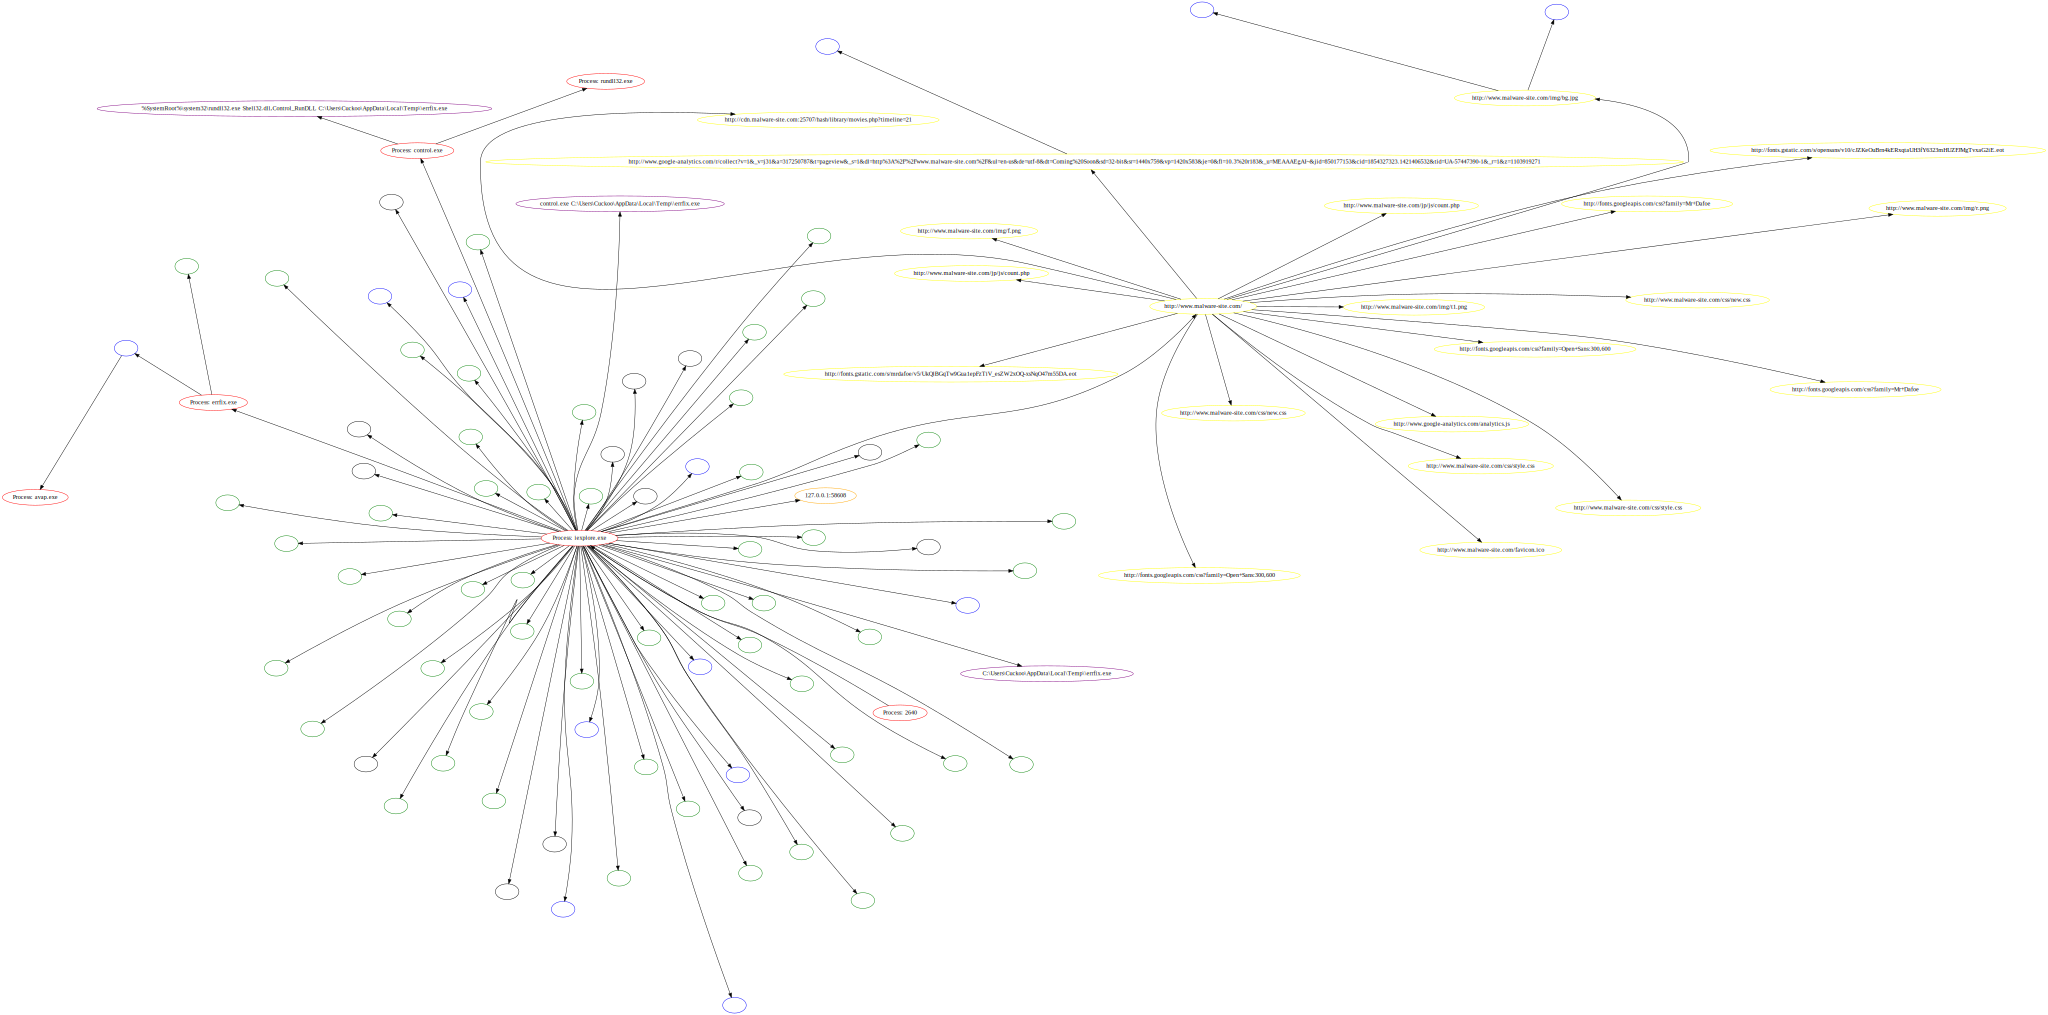
\includegraphics[width=25cm, angle=90]{Images/report_Subprocess_from_tab}
    \caption{An example of the subgraph where a single website was responsible for malware. For clarity, only the labels of visited URLs, involved processes and executed shell commands are shown.}
    \label{fig:subgraph}
\end{figure}

\stepcounter{savepage}
\pagebreak

\restoregeometry
\pagenumbering{arabic}
\setcounter{page}{\thesavepage}

\subsection{Comparison with Cuckoo 1.2}

To show the improvement which was made, several benchmarks where run with a different amount of URLs. Those benchmarks were compared with a development version of Cuckoo 1.2\footnote{\url{https://github.com/cuckoobox/cuckoo/commit/6177071cfd57500fbf1dc17a66f5aff39051c75e}}. This version was also used as the basis for our development. The benchmark consists of provisioning Cuckoo with one or more URLs until Cuckoo changes the status to ``reported''. Because the adapted version does not have this status, the benchmark stops when the \texttt{mass-analyse.py} script exits. Benchmarks were executed with 1, 5, 10, 25, 50 and 100 URLs. Each benchmark is run 25 times.\\

Figure \ref{fig:chart-box} shows a boxplot which compares the boxplot of the reference version with our modified version.\todo{Meer uitleg maar we hebben nog niet alle data} Figure \ref{fig:chart-trend} shows an interpolation and extrapolation of the results. The mean has been calculated over all results for a certain number of URLs.\\

In both of these figures, it can be seen that our version of Cuckoo is significantly better. For 1 URL, there is an improvement of 316\% and for more than 10 URLs, our version is at least ten times as fast.

The raw numbers used to generate these graphs can be found in Appendix B.\\

\todo{Boxplot voor elk aantal URLs voor reference Cuckoo}
\begin{figure}[h]
    \centering
    \centerline{\includegraphics[width=20cm]{Images/chart-box.png}}
    \caption{Boxplot}
    \label{fig:chart-box}
\end{figure}

\begin{figure}[h]
    \centering
    \centerline{\includegraphics[width=20cm]{Images/chart-trend}}
    \caption{Interpolation of the results. (Logaritmic scale)}
    \label{fig:chart-trend}
\end{figure}

\begin{table}[h]
\begin{tabular}{@{}lllllll@{}}
\toprule
                & 1 URL   & 5 URLs  & 10 URLs     & 25 URLs     & 50 URLs     & 100 URLs \\ \midrule
Reference       & 152,8   & 764,1   & 1528,2      & 3820,5      & 7640,9      & 15281,8 \\
Modified Cuckoo & 48,8    & 118,5   & 143,8       & 233,1       &             &         \\
Improvement     & 312,9\% & 644,6\% & 1062,6\%    & 1639,2\%    &             &         \\ \bottomrule
\end{tabular}
\end{table}
